\documentclass[a4paper,12pt]{article}
\usepackage[utf8x]{inputenc}
\usepackage [T1]{fontenc}
\usepackage{datetime}
\usepackage{indentfirst}
\usepackage{subcaption}
\usepackage{grffile}
\usepackage[section]{placeins}
\captionsetup{compatibility=false}

\usepackage[hmargin={20mm,10mm},vmargin={20mm,15mm},bindingoffset=0mm]{geometry}
\usepackage[colorlinks=true, linkcolor=blue, citecolor=blue, urlcolor=blue, unicode]{hyperref}


\usepackage{docstyle}

\begin{document}
\begin{titlepage}
	\centering
	{\scshape\large VILNIAUS UNIVERSITETAS \\
	MATEMATIKOS IR INFORMATIKOS FAKULTETAS \par}
	\vspace{6cm}
	{\huge\bfseries Žaidimų varikliuko kūrimas naudojant HTML5 galimybes\par}
	{\LARGE Tiriamojo seminaro ataskaita\par}
	{\Large Matematinė informatika 3 kursas}
	\vspace{3cm}
	\vfill
	\flushright
	Autorius: \\ Paulius Legeckas\par
	\vspace{0.5cm}
	Vadovas: \\ Irus Grinis
	\vfill
	\centering
	Vilnius\\
	{\the\year}
\end{titlepage}	
\tableofcontents

\newpage
\section*{Įvadas}


Nuo pat vaikystės žmonėms žaidimai yra viena patraukliausių laiko leidimo formų. Vaikams sudominti tėvai nuolat prigalvoja įvairių žaidimų kasdienėms nuobodžioms situacijoms, taip lengviau įtraukdamii į jų siūlomą veiklą. Toks būdas pritaikytas moksluose turi labai teigiamų rezultatų, todėl tokie dalykai kaip matematika ar informatika, kurie gali pasirodyti gana nuobodūs ir monotoniški, yra kur kas greičiau įsisavinami. Panašiu tikslu paremtas ir šis projektas, kur programavimas yra tiesiogiai sujungiamas su piešimu. \


\addcontentsline{toc}{section}{Įvadas}

\newpage
\section{Žaidimo variklio apibrėžimas}

Žaidimų variklis – programa įgalinanti vartotoją kurti bei vystyti kompiuterius ar mobilius žaidimus. Iš esmės tai yra įrankis palengvinantis darbą kūrėjui, kadangi jam pateikiamas interaktyvesnis būdas kurti tai, ko jis nori, nereikalaujant pernelyg gilių techninių žinių.\\

\section{Komenskio logo}

Komenskio Logo (Comenius logo ({\cite {Comenius logo}}) – interaktyvi programavimui skirta programa paremta Logo programavimo kalba. \\
Ši programa plačiai naudojama mokymo įstaigose norint padėti vaikams susipažinti bei geriau įsisavinti programavimo subtilybes. \\

Iš esmės ji remiasi vizualizacine kodo reprezentacija. Vartotojas rašydamas kodą gali judinti vežliuką, kuris eidamas palieka liniją ir taip piešia įvairius ornamentus kol galų gale gauna paveiksliuką. 

\begin{center}
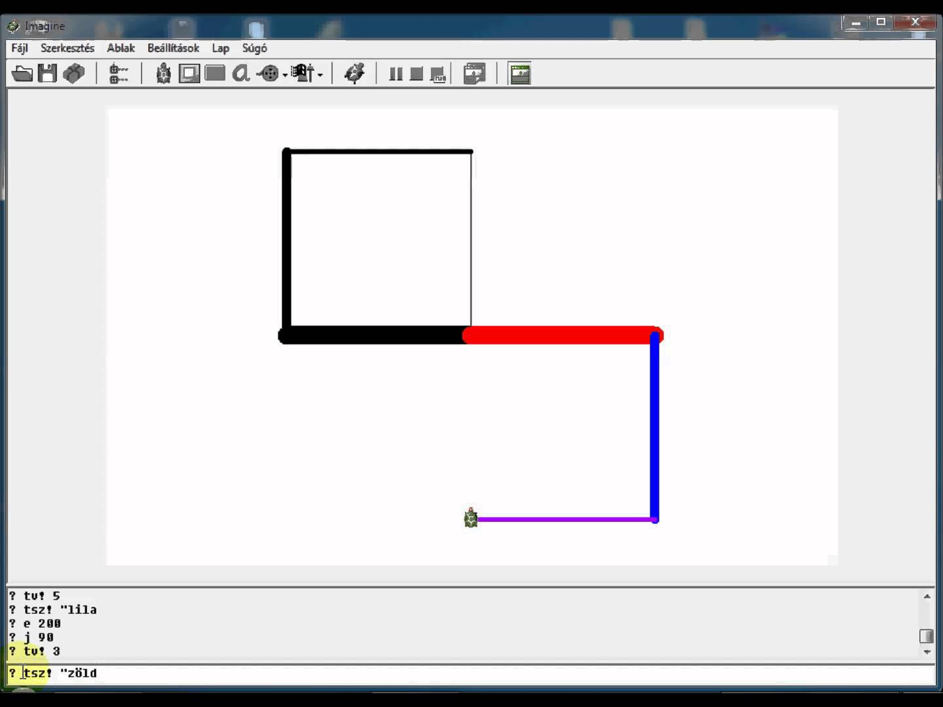
\includegraphics[scale=0.9]{LogoPvz1.png}\\
\textbf{Pav. 1}: Komenskio logo darbinis langas.\\
\end{center}

\newpage

\section{Galimybės}

Naudojantis komenskio logo galima sukurti įvairiausius 2d ornamentus, objektus ir juos sudėti į vieną paveiksliuką. \\

\begin{center}
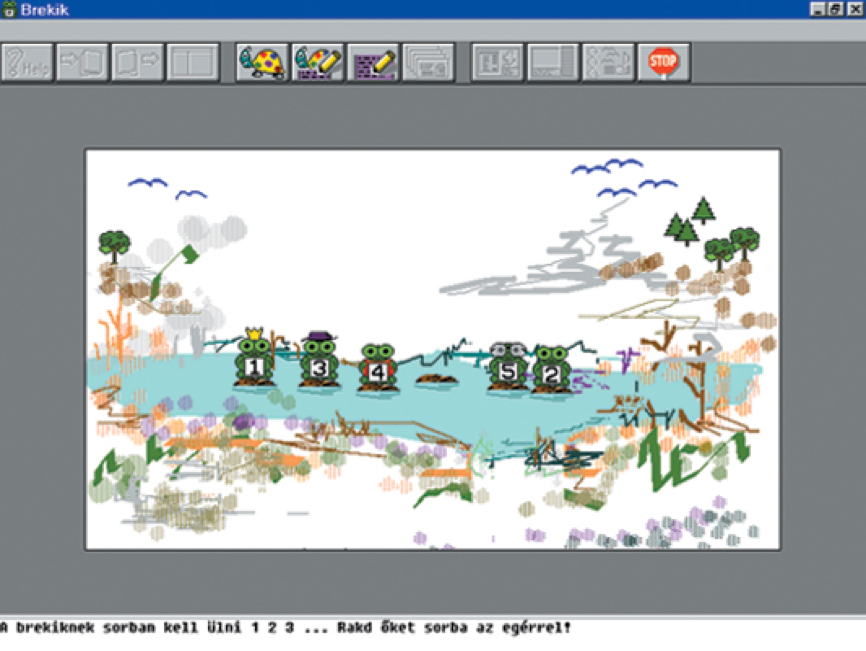
\includegraphics[scale=0.95]{LogoPiesinys1.png}\\
\textbf{Pav. 2}: Pavyzdinis piešinys.\\
\end{center}

\begin{center}
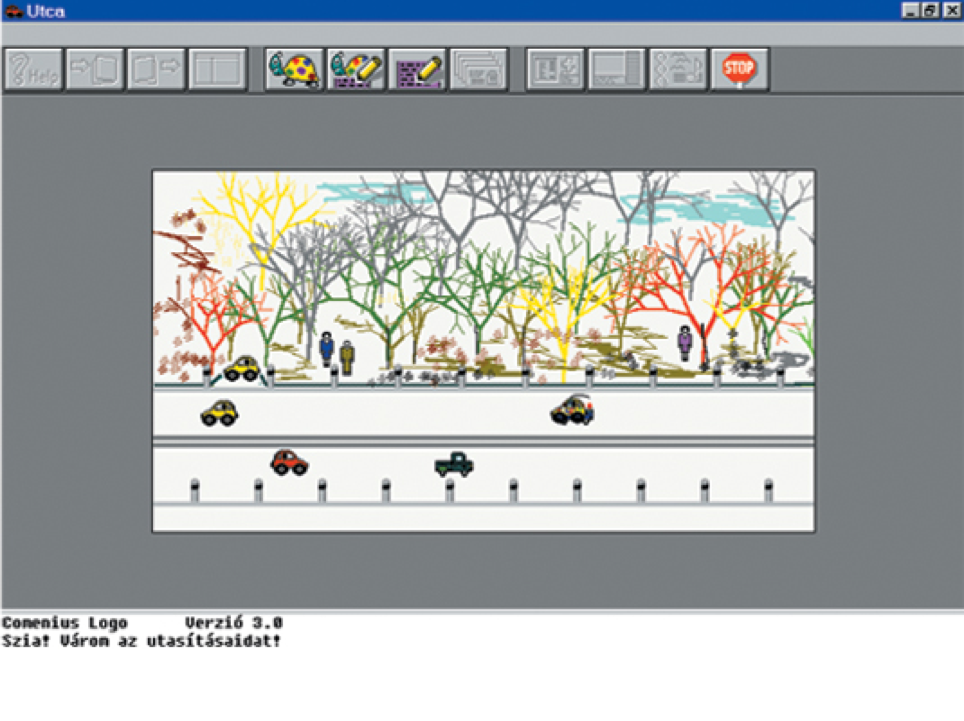
\includegraphics[scale=0.85]{LogoPiesinys2.png}\\
\textbf{Pav. 3}: Pavyzdinis piešinys (2).\\
\end{center}


\section{Projekto tikslas}

Mano projekto tikslas yra sukurti panašią alternatyvą, kuri būtų kiek modernesnė, lengvai prieinama internete bei turėtų galimybę išsaugoti bei persiųsti sukurtus piešinukus tarp vartotojų, juos būtų galima saugoti debesyse (cloud'e). \\

\section{Priemonės}

Šiam projektui sukurti naudojau NodeJS kalbą serverio kūrimui ir paleidimui, HTML5 bei Javascript kalbas variklio atvaizdavimui ir techninės dalies programavimui. \\

\section{Projekto stadija}

Šiuo metu vartotojas prisijungęs prie vietinio serverio (localhost) norėdamas pradėti piešti gali naudoti visas standartines funkcijas: eiti į priekį, atgal, pasisukti kairėn, dešinėn, pakelti bei nuleisti pieštuką, pakeisti pieštuko spalvą, storį, pakeisti vežliuko poziciją pagal koordinates, vietoj konstantų naudoti aritmetinius reiškinius ir pan.
Visą tai galima aprašyti ciklais, procedūromis bei kintamaisiais, kuriuos vos pora paspaudimų galima pakartotinai panaudoti. \\

\begin{center}
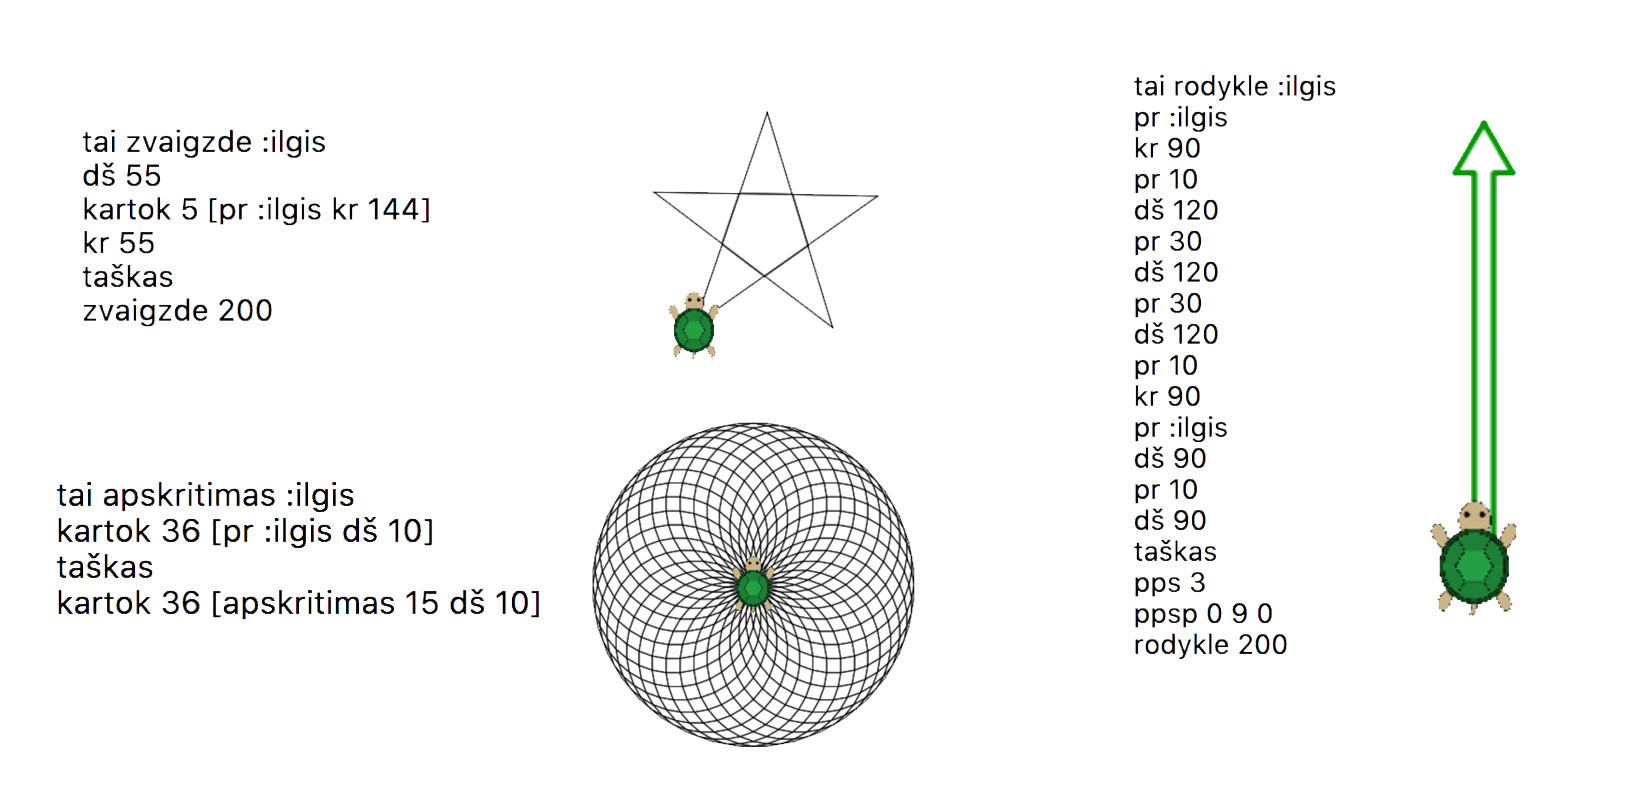
\includegraphics[scale=0.55]{ManoPvz1.png}\\
\textbf{Pav. 4}: Ornamentų pavyzdžiai su kodo atitikmenimis.\\
\end{center}

\begin{center}
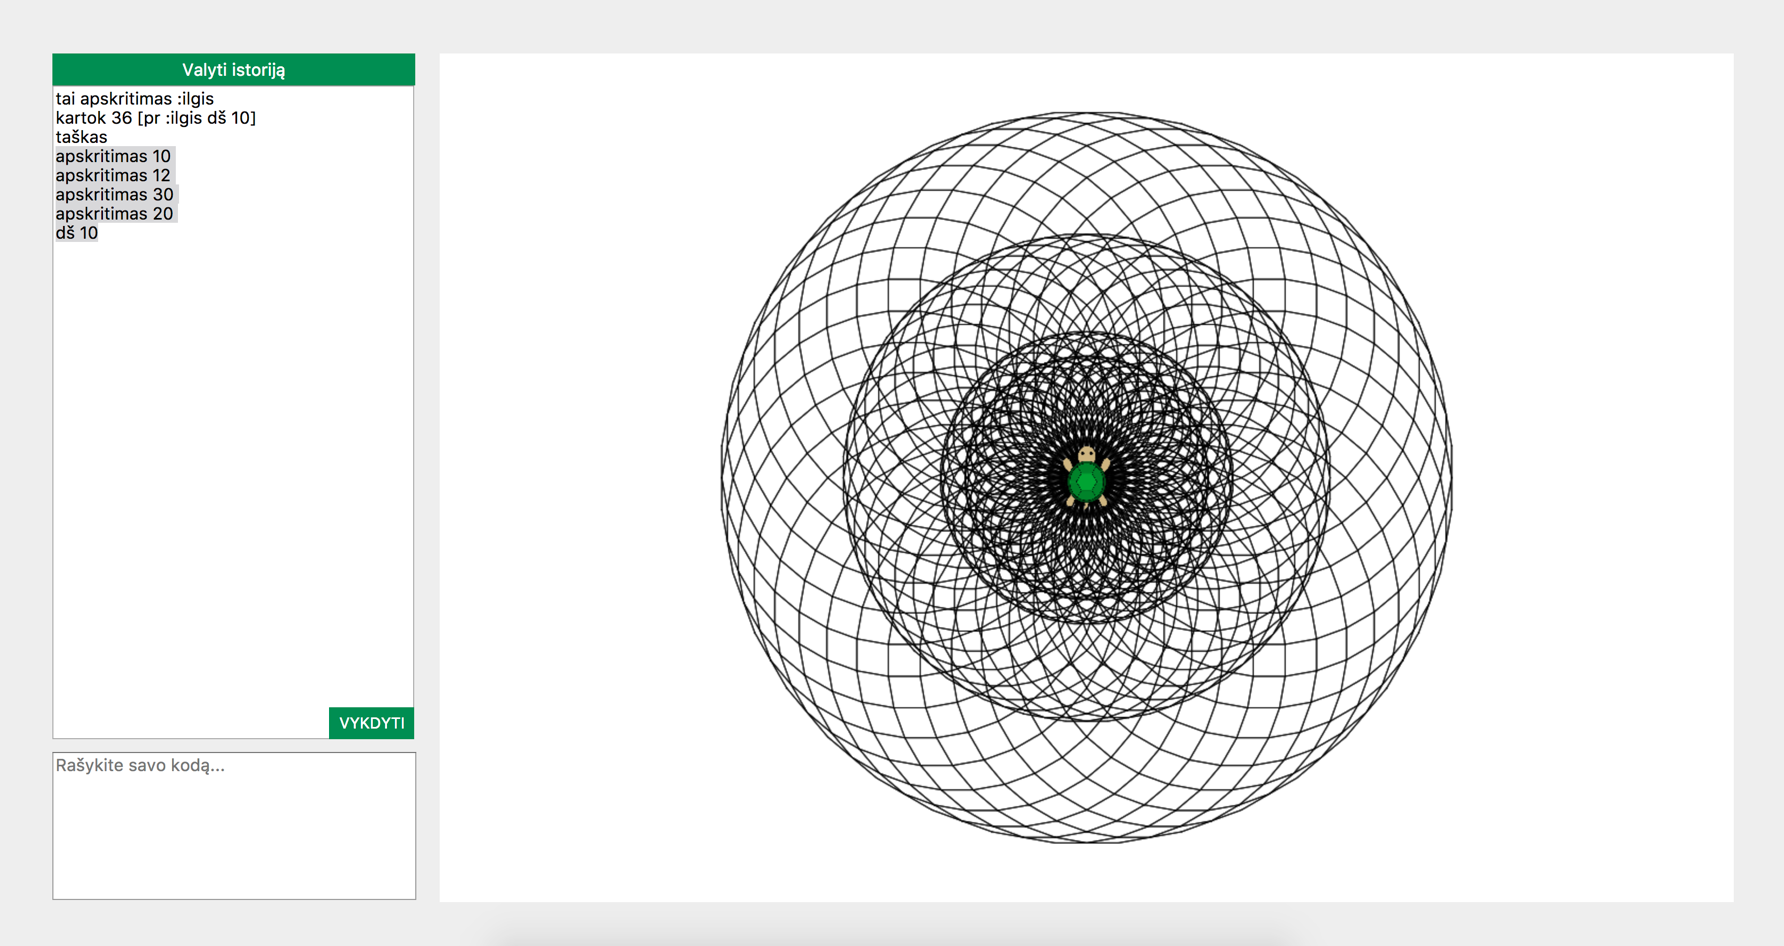
\includegraphics[scale=0.5]{ManoPvz2.png}\\
\textbf{Pav. 5}: Piešinio pavyzdys.\\
\end{center}

\begin{center}
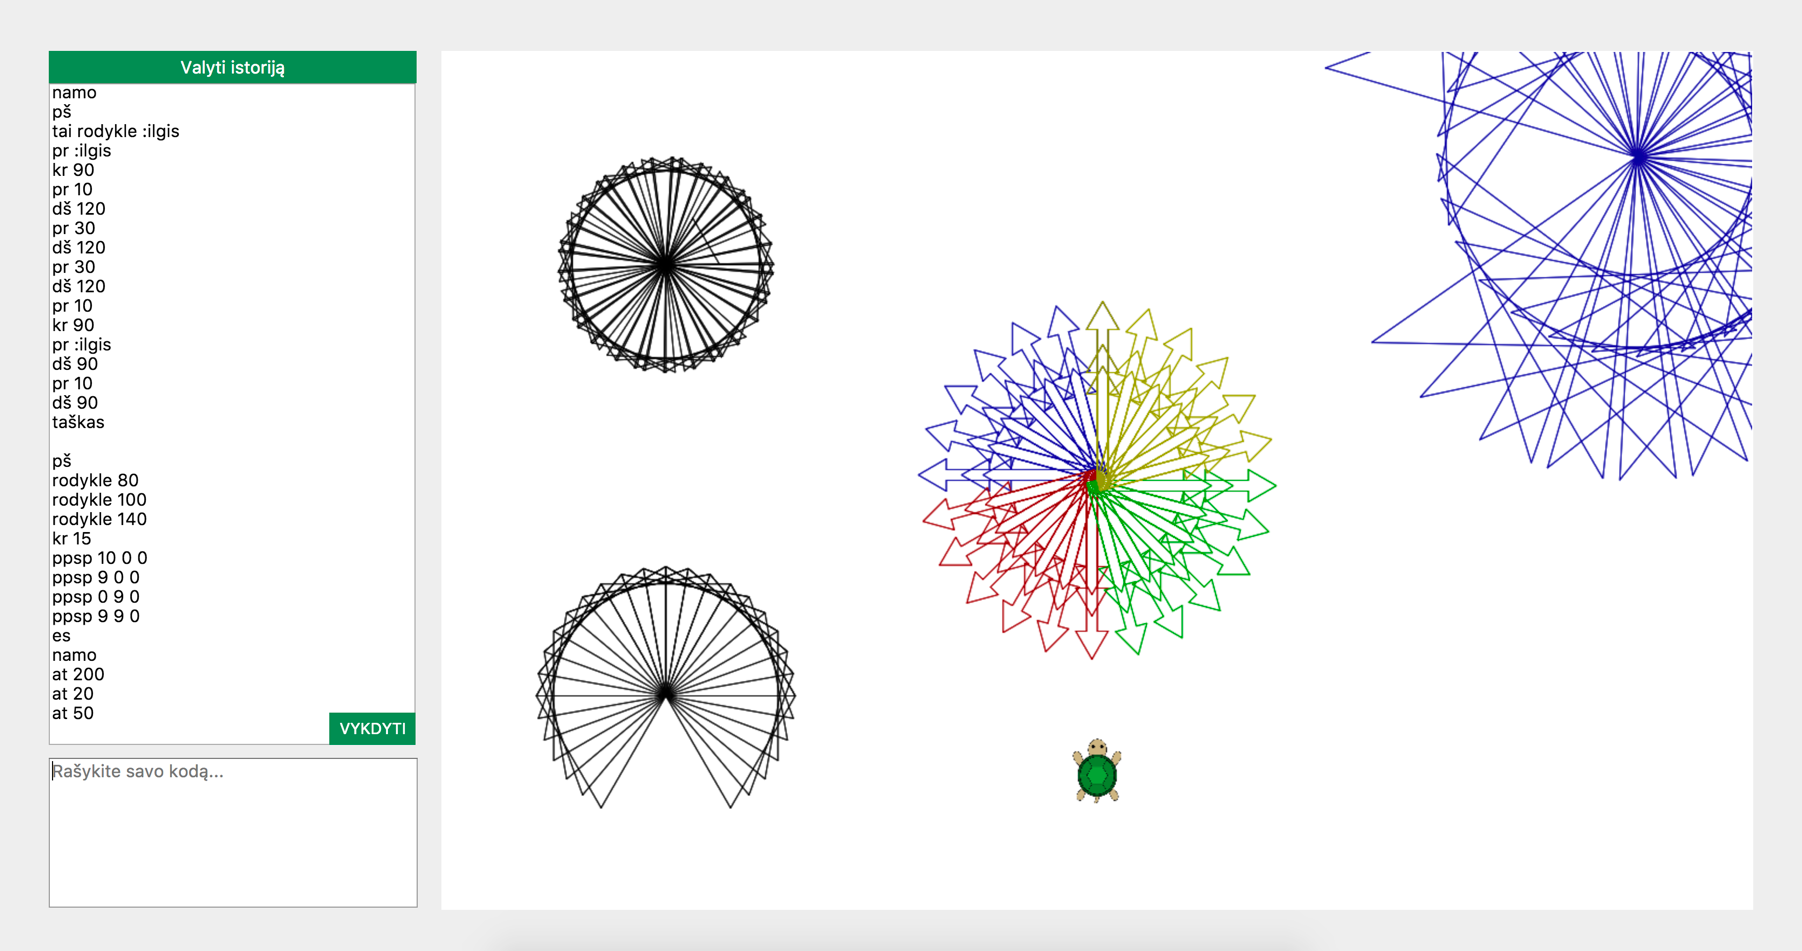
\includegraphics[scale=0.5]{ManoPvz3.png}\\
\textbf{Pav. 6}: Piešinio pavyzdys su skirtingomis spalvomis bei pieštuko storiu.\\
\end{center}

\section{Projekto ateitis}

Galų gale šis projektas turės panašų kiekį funkcionalumo kaip ir Komenskio Logo. Vartotojas galės susikurti savo kodu generuojamų ornamentų šablonus, jais dalintis su kitais. Programa bus pilnai nepriklausoma, veiks nuotoliniame serveryje. Vartotojai galės greitai prisijungti ir siųsti pranešimus tarpusavyje.  \

\newpage

\section*{Išvados}
\addcontentsline{toc}{section}{Išvados}


Taigi, per pastarąjį semestrą buvo įgyvendintas šio variklio pagrindas su standartinėmis piešimo komandomis. Šiuo metu didžiausias trūkumas yra pakankamai nedidelis funkcijų kiekis. Vartotojas norėdamas nupiešti sudetingesnį piešinį turėtų pritaikyti daugiau funkcijų nei leidžia šis variklis. Tačiau ateityje planuojama praplėsti šį funkcijų diapozoną ir kuo labiau palengvinti vartotojo darbą. \\

\renewcommand {\refname}{Literatūra}
\addcontentsline{toc}{section}{Literatūra}

\begin{thebibliography}{9}





\bibitem {Comenius logo} 
Komenskio logo pagrindinė svetainė URL: <
\url {http://harveycohen.net/oznaki/} >

\bibitem {Logo} 
Komenskio logo dokumentacija URL: <
\url {http://el.media.mit.edu/logo-foundation/what_is_logo/logo_programming.html} >

\bibitem {Knyga}
A, Blaho, I. Kalaš: Comenius Logo: tvoriva informatika, Vilnius, Žara, 2002, 356 psl.
\end{thebibliography}
\end{document}

